\documentclass[border=4pt]{standalone}

\usepackage{amsmath}
\usepackage{tikz}
\usepackage{mathdots}
\usepackage{yhmath}
\usepackage{cancel}
\usepackage{color}
\usepackage{siunitx}
\usepackage{array}
\usepackage{multirow}
\usepackage{amssymb}
\usepackage{gensymb}
\usepackage{tabularx}
\usepackage{booktabs}
\usetikzlibrary{fadings}
\usetikzlibrary{patterns}


\begin{document}
 




\tikzset{every picture/.style={line width=0.75pt}} %set default line width to 0.75pt        

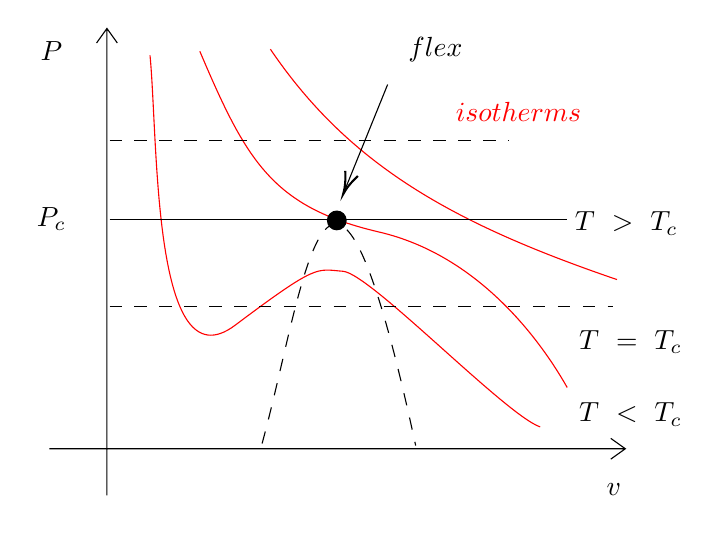
\begin{tikzpicture}[x=0.75pt,y=0.75pt,yscale=-1,xscale=1]
%uncomment if require: \path (0,300); %set diagram left start at 0, and has height of 300

%Shape: Axis 2D [id:dp21232904237515537] 
\draw  (41,226.5) -- (318.5,226.5)(68.75,24) -- (68.75,249) (311.5,221.5) -- (318.5,226.5) -- (311.5,231.5) (63.75,31) -- (68.75,24) -- (73.75,31)  ;
%Curve Lines [id:da27173483056318637] 
\draw   [color={rgb, 255:red, 255; green, 0; blue, 0 }  ,draw opacity=1 ]  (113.5,35) .. controls (136,88) and (148.5,110) .. (199.5,122) .. controls (247.5,133) and (277.5,174) .. (290.5,197) ;


%Curve Lines [id:da2848143995073411] 
\draw   [color={rgb, 255:red, 255; green, 0; blue, 0 }  ,draw opacity=1 ]  (89.5,37) .. controls (93.5,78) and (90.5,197) .. (130.5,167) .. controls (170.5,137) and (169.5,140) .. (182.5,141) .. controls (195.5,142) and (260.5,210) .. (277.5,216) ;


%Curve Lines [id:da802724207727525] 
\draw   [color={rgb, 255:red, 255; green, 0; blue, 0 }  ,draw opacity=1 ]  (147.5,34) .. controls (185.5,90) and (235.5,118) .. (314.5,145) ;


%Straight Lines [id:da027638903382105395] 
\draw    (204,51) -- (183.25,102.15) ;
\draw [shift={(182.5,104)}, rotate = 292.08] [color={rgb, 255:red, 0; green, 0; blue, 0 }  ][line width=0.75]    (10.93,-3.29) .. controls (6.95,-1.4) and (3.31,-0.3) .. (0,0) .. controls (3.31,0.3) and (6.95,1.4) .. (10.93,3.29)   ;

%Shape: Circle [id:dp619448912141028] 
\draw  [fill={rgb, 255:red, 0; green, 0; blue, 0 }  ,fill opacity=1 ] (175,116.5) .. controls (175,114.01) and (177.01,112) .. (179.5,112) .. controls (181.99,112) and (184,114.01) .. (184,116.5) .. controls (184,118.99) and (181.99,121) .. (179.5,121) .. controls (177.01,121) and (175,118.99) .. (175,116.5) -- cycle ;
%Curve Lines [id:da2790887134499407] 
\draw  [dash pattern={on 4.5pt off 4.5pt}]  (143.5,224) .. controls (164.5,147) and (175.5,30) .. (217.5,225) ;


%Straight Lines [id:da5692390174578967] 
\draw     [dash pattern={on 4.5pt off 4.5pt}]  (70,158) -- (312.5,158) ;

%Straight Lines [id:da5692390174578967] 
\draw     [dash pattern={on 4.5pt off 4.5pt}]  (70,78) -- (262.5,78) ;


%Straight Lines [id:da5692390174578967] 
\draw     (70,116) -- (290.5,116) ;

% Text Node
\draw (42,116) node   {$P_c$};

% Text Node
\draw (42,35) node   {$P$};
% Text Node
\draw (313,246) node   {$v$};
% Text Node
\draw (227,34) node   {$flex$};
% Text Node
\draw (319,118) node   {$T\  >\ T_{c}$};
% Text Node
\draw (321,175) node   {$T\ =\ T_{c}$};

% Text Node
\draw (321,210) node   {$T\ <\ T_{c}$};

% Text Node
\draw (267,64) node [color={rgb, 255:red, 255; green, 0; blue, 0 }  ,draw opacity=1 ]  {$isotherms$};

\end{tikzpicture}

\end{document}
